\documentclass[xcolor=dvipsnames,presentation]{beamer}    % ,handout
% colortbl only defines \rowcolor for a single row. xcolor extends this to multiple rows.

\usetheme[sectionoutline]{Aachen} %
\usepackage[ngerman]{babel}
\usepackage[T1]{fontenc}
\usepackage[utf8]{inputenc}


%%%%%%%%%%%%%%%%%%%%%%%%%%%%%%%%%%%%%%%%%%%%%%%%%%%%%%%%%%%%%%%%%%%%%%
% tables
\usepackage{multirow,array,tabularx,rotating}
\usepackage{booktabs}

% math
\usepackage{amsmath,amsthm, amssymb, latexsym, xspace}
\usepackage{bbold}
%\usefonttheme[onlymath]{serif}
%\boldmath

% misc
\usepackage{subfigure}
\usepackage{wasysym}
\usepackage{nameref}

\usepackage{tikz}
\usetikzlibrary{trees,calc}
\usepackage[absolute,overlay]{textpos}

\tikzset{
grow=down,
level 1/.style={sibling distance=7cm, level distance=3cm},
level 2/.style={sibling distance=7cm, level distance=3cm},
level 3/.style={sibling distance=7cm, level distance=3cm},
level 4/.style={sibling distance=7cm, level distance=3cm},
virtual/.style={ultra thick,rectangle,draw=black},
leaf/.style={ultra thick,circle,draw=black},
edge from parent/.style={ultra thick,draw=black},
edge from parent path={
(\tikzparentnode) |-
($(\tikzparentnode)!0.5!(\tikzchildnode)$) -|
(\tikzchildnode)},
}

\tikzstyle{end} = [circle, minimum width=15pt, fill, inner sep=0pt]

\renewcommand*\ttdefault{txtt}


% declare the path(s) where your graphic files are
\graphicspath{./bilder/}
% and their extensions so you won't have to specify these with
% every instance of \includegraphics
\DeclareGraphicsExtensions{.pdf,.jpeg,.png}

% helpers
\newcommand{\argmin}{\operatornamewithlimits{argmin}}
\newcommand{\argmax}{\operatornamewithlimits{argmax}}

%%%%%%%%%%%%%%%%%%%%%%%%%%%%%%%%%%%%%%%%%%%%%%%%%%%%%%%%%%%%%%%%%%%%%%
%%%%%%%%%%%%%%%%%%%%%%%%%%%%%%%%%%%%%%%%%%%%%%%%%%%%%%%%%%%%%%%%%%%%%%

\renewcommand*{\email}{\url{thomas.gatzweiler@rwth-aachen.de}}
% all email address(es) of the authors (used for \TitlePage)

\title[Adaptive Huffman-Kodierung und Anwendungen]{Adaptive Huffman-Kodierung und Anwendugen}

\setbeamertemplate{navigation symbols}{} %disable navigation bar

%% author and in []: shortauthor
\author[Gatzweiler]{Thomas Gatzweiler}
% - Use the \inst{?} command only if the authors have different
%   affiliation.
\institute[RWTH Aachen University] % (optional, but mostly needed)
{
%  \inst{1}%
  \strut Human Language Technology and Pattern Recognition\\
  \strut Computer Science Department, RWTH Aachen University %\\
  %\strut {\tt lehnen@cs.rwth-aachen.de}
}
% - Use the \inst command only if there are several affiliations.
% - Keep it simple, no one is interested in your street address.

\date[12. November 2014]{Proseminar Datenkompression, 12. November 2014, Aachen}

%%%%%%%%%%%%%%%%%%%%%%%%%%%%%%%%%%%%%%%%%%%%%%%%%%%%%%%%%%%%%%%%%%%%%%
% will be set into the PDF document summary
\hypersetup{
  pdftitle={\inserttitle}, 
  pdfauthor={\insertauthor}, 
  bookmarksdepth=subsubsection,  
  % enable automatic page transitions: for endless loop edit in
  % acrobat reader -> preferences -> full screen -> after every X
  % seconds and after last page
  %pdfpageduration = 2, 
  % pdfpagetransition = {Glitter /Di 315 /D 5}  
  % pdfpagetransition = {Box /M /O /D 1},
}

%%%%%%%%%%%%%%%%%%%%%%%%%%%%%%%%%%%%%%%%%%%%%%%%%%%%%%%%%%%%%%%%%%%%%%
\usepackage{pdfpcnotes}

%%%%%%%%%%%%%%%%%%%%%%%%%%%%%%%%%%%%%%%%%%%%%%%%%%%%%%%%%%%%%%%%%%%%%%
%%%%%%%%%%%%%%%%%%%%%%%%%%%%%%%%%%%%%%%%%%%%%%%%%%%%%%%%%%%%%%%%%%%%%%

\newenvironment{witemize}{\itemize\setlength{\itemsep}{1em}}{\enditemize}

%%%%%%%%%%%%%%%%%%%%%%%%%%%%%%%%%%%%%%%%%%%%%%%%%%%%%%%%%%%%%%%%%%%%%%
%%%%%%%%%%%%%%%%%%%%%%%%%%%%%%%%%%%%%%%%%%%%%%%%%%%%%%%%%%%%%%%%%%%%%%
\begin{document}
% Literaturverzeichnis wie in der .bib Datei ordnen
\nocite{*}

%%%%%%%%%%%%%%%%%%%%%%%%%%%%%%%%%%%%%%%%%%%%%%%%%%%%%%%%%%%%%%%%%%%%%%
\begin{frame}[label=titlepage]
  \titlepage
\end{frame}

%%%%%%%%%%%%%%%%%%%%%%%%%%%%%%%%%%%%%%%%%%%%%%%%%%%%%%%%%%%%%%%%%%%%%%

% use this, if you use option nosectionoutline
%
% \begin{frame}<*>{\iflanguage{ngerman}{Gliederung}{Outline}}
%       \tableofcontents[subsectionstyle=show/show/show]
% \end{frame}

%%%%%%%%%%%%%%%%%%%%%%%%%%%%%%%%%%%%%%%%%%%%%%%%%%%%%%%%%%%%%%%%%%%%%%

%\section{Einführung} \label{sec:intro}
%\begin{frame}{\insertsection}
%Hello World
%\pnote{bla bla bla}
%\end{frame}

%%%%%%%%%%%%%%%%%%%%%%%%%%%%%%%%%%%%%%%%%%%%%%%%%%%%%%%%%%%%%%%%%%%%%%

\begin{frame}[allowframebreaks]{Literatur}
 %\bibliographystyle{alpha}
 \bibliographystyle{i6bibliostyle}
 \bibliography{references}
\end{frame}

%%%%%%%%%%%%%%%%%%%%%%%%%%%%%%%%%%%%%%%%%%%%%%%%%%%%%%%%%%%%%%%%%%%%%%

\section{Huffman-Kodierung}

\begin{frame}[<+->]{\insertsection}
  \pnote{Grundlage für die adaptive Huffman-Kodierung}
  \begin{witemize}
    \item 1952 von David Huffman entwickelt
    \item Erzeugt einen präfixfreien Code
      \begin{itemize}
        \item{Kein Codewort ist Präfix eines anderen Codeworts}
      \end{itemize}
      \pnote{Vorteil: Codewörter lassen sich direkt hintereinander schreiben}
    \item Entropiekodierung
      \begin{itemize}
        \item Häufige Symbole $\Rightarrow$ Kurze Codewörter
        \item Seltene Symbole $\Rightarrow$ Lange Codewörter
      \end{itemize}
    \item Verlustfreie Komprimierung
  \end{witemize}
\end{frame}

\subsection{Huffman-Baum}

\begin{frame}[<+->]{\insertsubsection}
  \begin{witemize}
  \item Zentrale Datenstruktur für Kodierung und Dekodierung
  \item Binärbaum zur Erzeugung eines binären Codes
    \pnote{Lässt sich auch auf andere Zahlensysteme anwenden}
  \item Wahrscheinlichkeitsverteilung des Eingabealphabets muss bekannt sein
    \pnote{Wahrscheinlichkeiten können geschätzt oder vorher ermittelt werden}
  \item Aufbau von des Baums unten nach oben
    \pnote{Kodierung ist präfixfrei, da die Symbole nur in den Blättern stehen}
  \end{witemize}
\end{frame}

\begin{frame}[<+->]{\insertsubsection: Konstruktion}
  \begin{witemize}
  \item Sortierung der Liste des Eingabealphabets nach Wahrscheinlichkeiten
  \item Die zwei seltensten Symbole werden aus der Liste entfernt
  \item Erzeugung je eines Blattknotens für die zwei Symbole
  \item Erzeugung eines Elternknotens für die zwei Blattknoten
  \item Einfügen eines Hilfssymbols mit der summiertern
    Wahrscheinlichkeit beider Symbole in die Liste
  \item Wiederholung bis ein Hilfssymbol übrig bleibt
  \end{witemize}
\end{frame}

\begin{frame}[fragile]{\insertsubsection: Beispiel}

\begin{textblock}{5}(10,3)
\begin{flushright}
\begin{tabular}{l|l}
$a_i$ & $P(a_i)$ \\ \hline
\only<1>
{A & 0.20 \\
B & 0.06 \\
C & 0.10 \\
D & 0.14 \\
E & 0.50}\only<2>
{E & 0.50 \\
A & 0.20 \\
D & 0.14 \\
C & 0.10 \\
B & 0.06}\only<3-4>
{E & 0.50 \\
A & 0.20 \\
D & 0.14 \\
\color{red}C & \color{red}0.10 \\
\color{red}B & \color{red}0.06}\only<5>
{E & 0.50 \\
A & 0.20 \\
\color{ForestGreen}\{C, B\} & \color{ForestGreen}0.16 \\
D & 0.14}\only<6-7>
{E & 0.50 \\
A & 0.20 \\
\color{red}\{C, B\} & \color{red}0.16 \\
\color{red}D & \color{red}0.14}\only<8>
{E & 0.50 \\
\color{ForestGreen}\{B, C, D\} & \color{ForestGreen}0.30 \\
A & 0.20}\only<9-10>
{E & 0.50 \\
\color{red}\{B, C, D\} & \color{red}0.30 \\
\color{red}A & \color{red}0.20}\only<11>
{E & 0.50 \\
\color{ForestGreen}\{A, B, C, D\} & \color{ForestGreen}0.50}\only<12-13>
{\color{red}E & \color{red}0.50 \\
\color{red}\{A, B, C, D\} & \color{red}0.50}\only<14-15>
{\color{ForestGreen}\{A, B, C, D, E\} & \color{ForestGreen}1.00}
\end{tabular}
\end{flushright}
\end{textblock}

\begin{tikzpicture}[
level 1/.style={sibling distance=8cm, level distance=3.5cm},
level 2/.style={sibling distance=6cm, level distance=3.5cm},
level 3/.style={sibling distance=6cm, level distance=3.5cm},
level 4/.style={sibling distance=6cm, level distance=3.5cm},
]
\tikzstyle{lvl8}=[transparent]
\tikzstyle{lvl7}=[transparent]
\tikzstyle{lvl6}=[transparent]
\tikzstyle{lvl5}=[transparent]
\tikzstyle{lvl4}=[transparent]
\tikzstyle{lvl3}=[transparent]
\tikzstyle{lvl2}=[transparent]
\tikzstyle{lvl1}=[transparent]
\tikzstyle{lvl0}=[transparent]
\only<4->{\tikzstyle{lvl0}=[opaque]}
\only<5->{\tikzstyle{lvl1}=[opaque]}
\only<7->{\tikzstyle{lvl2}=[opaque]}
\only<8->{\tikzstyle{lvl3}=[opaque]}
\only<10->{\tikzstyle{lvl4}=[opaque]}
\only<11->{\tikzstyle{lvl5}=[opaque]}
\only<13->{\tikzstyle{lvl6}=[opaque]}
\only<14->{\tikzstyle{lvl7}=[opaque]}
\only<15->{\tikzstyle{lvl8}=[opaque]}
\node[virtual,lvl7] {\{A, B, C, D, E\}}
child[lvl6] {
  node[leaf] {E}
  edge from parent
  node[left,lvl8] {\small$0.50$}
}
child[lvl6] {
  node[virtual,lvl5] {\{A, B, C, D\}}
  child[lvl4] {
    node[virtual,lvl3] {\{B, C, D\}}
    child[lvl2] {
      node[virtual,lvl1] {\{C, B\}}
      child[lvl0] {
        node[leaf] {C}
        edge from parent
        node[left,lvl8] {\small$0.10$}
      }
      child[lvl0] {
        node[leaf] {B}
        edge from parent
        node[right,lvl8] {\small$0.06$}
      }
      edge from parent
      node[left,lvl8] {\small$0.16$}
    }
    child[lvl2] {
      node[leaf] {D}
      edge from parent
      node[right,lvl8] {\small$0.14$}
    }
    edge from parent
    node[left,lvl8] {\small$0.30$}
  }
  child[lvl4] {
    node[leaf] {A}
    edge from parent
    node[right,lvl8] {\small$0.20$}
  }
  edge from parent
  node[right,lvl8] {\small$0.50$}
};
\end{tikzpicture}
\end{frame}

\subsection{Kodierung}

\begin{frame}[<+->]{\insertsubsection}
  \begin{witemize}
  \item Codewort-Erzeugung aus dem Pfad von der Wurzel zum Blatt
    \begin{itemize}
    \item Linker Teilbaum: {\tt1} wird angehängt
    \item Rechter Teilbaum: {\tt0} wird angehängt
    \item Oder umgekehrt (Implementationsabhängig)
    \end{itemize}
  \end{witemize}
\end{frame}

\begin{frame}{\insertsubsection: Beispiel}
\begin{textblock}{5}(10,3)
\begin{flushright}
\begin{tabular}{l|l}
$a_i$ & $C(a_i)$ \\ \hline
\only<2->
{\only<2>{\color{i6blue}}A & \only<2>{\color{i6blue}}{\tt00} \\}
\only<3->
{\only<3>{\color{i6blue}}B & \only<3>{\color{i6blue}}{\tt0110} \\}
\only<4->
{\only<4>{\color{i6blue}}C & \only<4>{\color{i6blue}}{\tt0111} \\}
\only<5->
{\only<5>{\color{i6blue}}D & \only<5>{\color{i6blue}}{\tt010} \\}
\only<6->
{\only<6>{\color{i6blue}}E & \only<6>{\color{i6blue}}{\tt1} \\}
\end{tabular}
\end{flushright}
\end{textblock}

\only<8-9>{
\begin{textblock}{8}(9,12)
$C(EBBE) = \only<9>{\tt1011001101}$
\end{textblock}
}

\begin{tikzpicture}[
level 1/.style={sibling distance=8cm, level distance=3.5cm},
level 2/.style={sibling distance=6cm, level distance=3.5cm},
level 3/.style={sibling distance=6cm, level distance=3.5cm},
level 4/.style={sibling distance=6cm, level distance=3.5cm},
]
\tikzstyle{A}=[]
\tikzstyle{B}=[]
\tikzstyle{C}=[]
\tikzstyle{D}=[]
\tikzstyle{E}=[]
\only<2>{\tikzstyle{A}=[i6blue,line width=8pt]}
\only<3>{\tikzstyle{B}=[i6blue,line width=8pt]}
\only<4>{\tikzstyle{C}=[i6blue,line width=8pt]}
\only<5>{\tikzstyle{D}=[i6blue,line width=8pt]}
\only<6>{\tikzstyle{E}=[i6blue,line width=8pt]}
\node[virtual] {\{A, B, C, D, E\}}
child {
  node[leaf] {E}
  edge from parent[E]
  node[left] {\tt1}
}
child {
  node[virtual] {\{A, B, C, D\}}
  child {
    node[virtual] {\{B, C, D\}}
    child {
      node[virtual] {\{C, B\}}
      child {
        node[leaf] {C}
        edge from parent[C]
        node[left] {\tt1}
      }
      child {
        node[leaf] {B}
        edge from parent[B]
        node[right] {\tt0}
      }
      edge from parent[B,C]
      node[left] {\tt1}
    }
    child {
      node[leaf] {D}
      edge from parent[D]
      node[right] {\tt0}
    }
    edge from parent[B,C,D]
    node[left] {\tt1}
  }
  child {
    node[leaf] {A}
    edge from parent[A]
    node[right] {\tt0}
  }
  edge from parent[A,B,C,D]
  node[right] {\tt0}
};
\end{tikzpicture}
\end{frame}

\subsection{Dekodierung}

\begin{frame}[<+->]{\insertsubsection}
  \begin{witemize}
  \item Huffman-Baum oder Wahrscheinlichkeitsverteilung wird benötigt
  \item Aufbau des Huffman-Baums genau wie beim Kodierer
  \item Dekodierer startet bei der Wurzel, ließt die Daten bitweise
    \begin{itemize}
    \item {\tt1} eingelesen: Zum linken Nachfolger gehen
    \item {\tt0} eingelesen: Zum rechten Nachfolger gehen
    \item Oder umgekehrt (gleiches Verhalten wie beim Kodierer notwendig)
    \end{itemize}
  \item Blatt erreicht: Symbol ausgeben und zur Wurzel zurückkehren
  \end{witemize}
\end{frame}

\section{Adaptive Huffman-Kodierung}

\begin{frame}[<+->]{\insertsection}
  \begin{witemize}
  \item Huffman-Kodierung:
    \begin{itemize}
      \item Wahrscheinlichkeitsverteilung muss
        bekannt sein
      \item Bestimmung in zusätzlichem Durchgang
      \item Echtzeitkodierung nicht möglich
    \end{itemize}
  \item Lösung: Adaptive Huffman-Kodierung
    \begin{itemize}
    \item 1973 von Newton Faller und 1978 von Robert Gallager
      unabhängig entwickelt
    \item 1985 von Donald Knuth wesentlich verbessert
    \item Basiert auf der Huffman-Kodierung
    \item Kodierung ohne Verzögerung, in einem Durchgang
    \item Jedes Eingangssymbol erzeugt sofort ein Codewort
    \item Passt sich laufend der Häufigkeitsverteilung an
    \end{itemize}
  \end{witemize}
\end{frame}

\begin{frame}[<+->]{\insertsection}
  \begin{witemize}
  \item Start mit leerem Huffman-Baum
  \item Knoten haben Häufigkeitszähler (Integer)
  \item Aktualisierung des Huffman-Baums bei neuen Eingabesymbolen und
    neuer Häufigkeitsverteilung
  \item Kodierer und Dekodierer müssen Operationen auf den
    Huffman-Baum exakt spiegeln
  \end{witemize}
\end{frame}

\subsection{Kodierung}

\begin{frame}[<+->]{\insertsubsection}
  \begin{witemize}
  \item Unbekannte Symbole:
    \begin{itemize}
    \item In den Huffman-Baum einfügen
    \item Unkodiert ausgeben
    \end{itemize}

  \item Bekannte Symbole:
    \begin{itemize}
    \item Codewort ausgeben
    \item Huffman-Baum aktualisieren
    \end{itemize}
  \end{witemize}
\end{frame}

\subsection{Dekodierung}

\begin{frame}[<+->]{\insertsubsection}
  \begin{witemize}
  \item Spiegelt die Änderungen des Huffman-Baums vom Kodierer
  \item Unkomprimiertes Symbol:
    \begin{itemize}
      \item In den Huffman-Baum einfügen
      \item Direkt wieder ausgeben
    \end{itemize}
  \item Komprimiertes Symbol:
    \begin{itemize}
      \item Dekodiertes Symbol ausgeben
      \item Huffman-Baum aktualisieren
    \end{itemize}
  \end{witemize}
\end{frame}

\begin{frame}[<+->]{\insertsection}
  \begin{witemize}
    \item Wie kann der Dekodierer zwischen Codewörtern und unkodierten
      Symbolen unterscheiden?
    \item Lösung: Benutzung eines Escape-Codes
    \item Neues Problem:
      \begin{itemize}
      \item Escape-Code darf kein Codewort und kein Präfix davon sein
      \item Codewörter ändern sich laufend
      \end{itemize}
    \item Lösung: Escape-Code als Symbol im Huffman-Baum verwalten
      \pnote{Codewort des Escape-Codes passt sich automatisch der
        Häufigkeit neuer Symbole an}
  \end{witemize}
\end{frame}

\begin{frame}[<+->]{Escape-Code im Huffman-Baum}
\begin{figure}
\begin{tikzpicture}
\node {}
child {
  node[leaf] {A}
  edge from parent
  node[left]  {\tt1}
}
child {
  child {
    node[leaf] {B}
    edge from parent
    node[left] {\tt1}
  }
  child {
    child {
      node[end] {}
      edge from parent
      node[left] {\tt1}
    }
    child {
      node[leaf] {C}
      edge from parent
      node[right] {\tt0}
    }
    edge from parent
    node[right] {\tt0}
  }
  edge from parent
  node[right] {\tt0}
};
\end{tikzpicture}
\end{figure}
Escape-Code: {\tt001}
\end{frame}

\subsection{Aktualisierung des Huffman-Baums}

\begin{frame}[<+->]{\insertsubsection}
  \begin{witemize}
  \item Huffman-Baum muss nach jeder Aktualisierung geprüft werden
    \item Häufigkeiten müssen monoton steigend sein, von links unten nach
      rechts oben
  \item Wenn notwendig Huffman-Baum ändern
  \end{witemize}
\end{frame}

\begin{frame}[<+->]{\insertsubsection: Algorithmus}
  Der Häufigkeitszähler $F$ von Blattknoten $X$ soll inkrementiert werden.

  \vspace{1cm}

  \begin{enumerate}
  \item Existiert von links unten nach rechts oben gesehen ein
    Nachfolger von $X$ mit einem Häufigkeitszähler $\leq F$, tausche
    $X$ mit dem letzen dieser Nachfolger.

    \emph{Ausnahme:} $X$ darf nicht mit dem Elternknoten getauscht werden
  \item Inkrementiere den Häufigkeitszähler des Knotens $X$ von $F$ auf $F+1$

  \item Ist $X$ der Wurzelknoten, stoppe die Ausführung, sonst führe
    den Algorithmus auf dem Elternknoten von $X$ aus.
  \end{enumerate}
\end{frame}

\subsection{Überlauf der Häufigkeitszähler}

\begin{frame}[<+->]{\insertsubsection}
  \begin{witemize}
  \item Häufigkeitszähler werden als Integer gespeichert
  \item Große Datenmengen können zum Integerüberlauf führen
  \item Lösung: Skalierung der Häufigkeitszähler zur Verhinderung
    \begin{itemize}
    \item Häufgkeitszähler werden durch 2 geteilt $\Rightarrow$ Right-Shift
    \item Huffmanbaum muss evtl. neu geordnet werden
    \end{itemize}
  \end{witemize}
\end{frame}

\section{Anwendungen}

\begin{frame}[<+->]{\insertsection}
  \begin{witemize}
  \item Huffman-Kodierung wird meist adaptiv verwendet
  \item Häufig Teil eines mehrstufigen Prozesses
  \item Beispiele:
    \begin{itemize}
    \item Unix-Tool {\tt{compact}}
    \item Letzte Stufe der JPEG-Komprimierung
    \item Teil der MP3- und AAC-Komprimierung
    \end{itemize}
  \end{witemize}
\end{frame}

\subsection{Textkompression}

\begin{frame}[<+->]{\insertsubsection}

\end{frame}

\subsection{Bildkompression}

\begin{frame}[<+->]{\insertsubsection}
\begin{witemize}
\item Keine Kompression bei 1-Bit Schwarz-Weiß-Bildern möglich
  \begin{itemize}
    \item {\tt0}: Schwarz, {\tt1}: Weiß
  \end{itemize}

\item Einfachster Fall: 8-Bit Graustufenbilder
  \begin{itemize}
    \item {\tt0}: Schwarz, {\tt1-254}: Graustufen, {\tt255}: Weiß
  \end{itemize}

\item Farbbilder
  \begin{itemize}
    \item Ein Huffman-Baum pro Farbkanal möglich
    \item Korrelation zwischen Farbkanälen bleibt unberücksichtigt
  \end{itemize}
\end{witemize}
\end{frame}

\begin{frame}{\insertsubsection}
\begin{figure}[T]
  \centering
  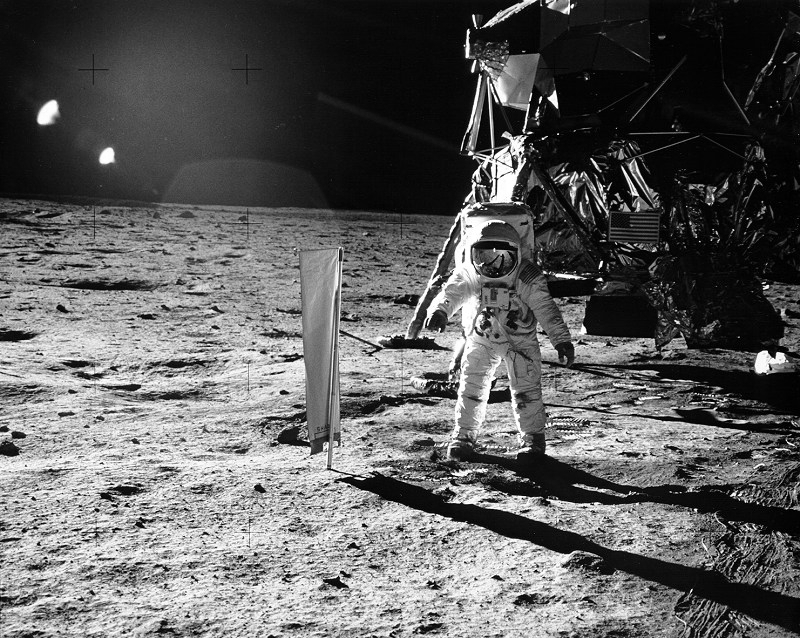
\includegraphics[width=0.470\textwidth]{bilder/moon.jpg}
  \hfill
  \only<2>{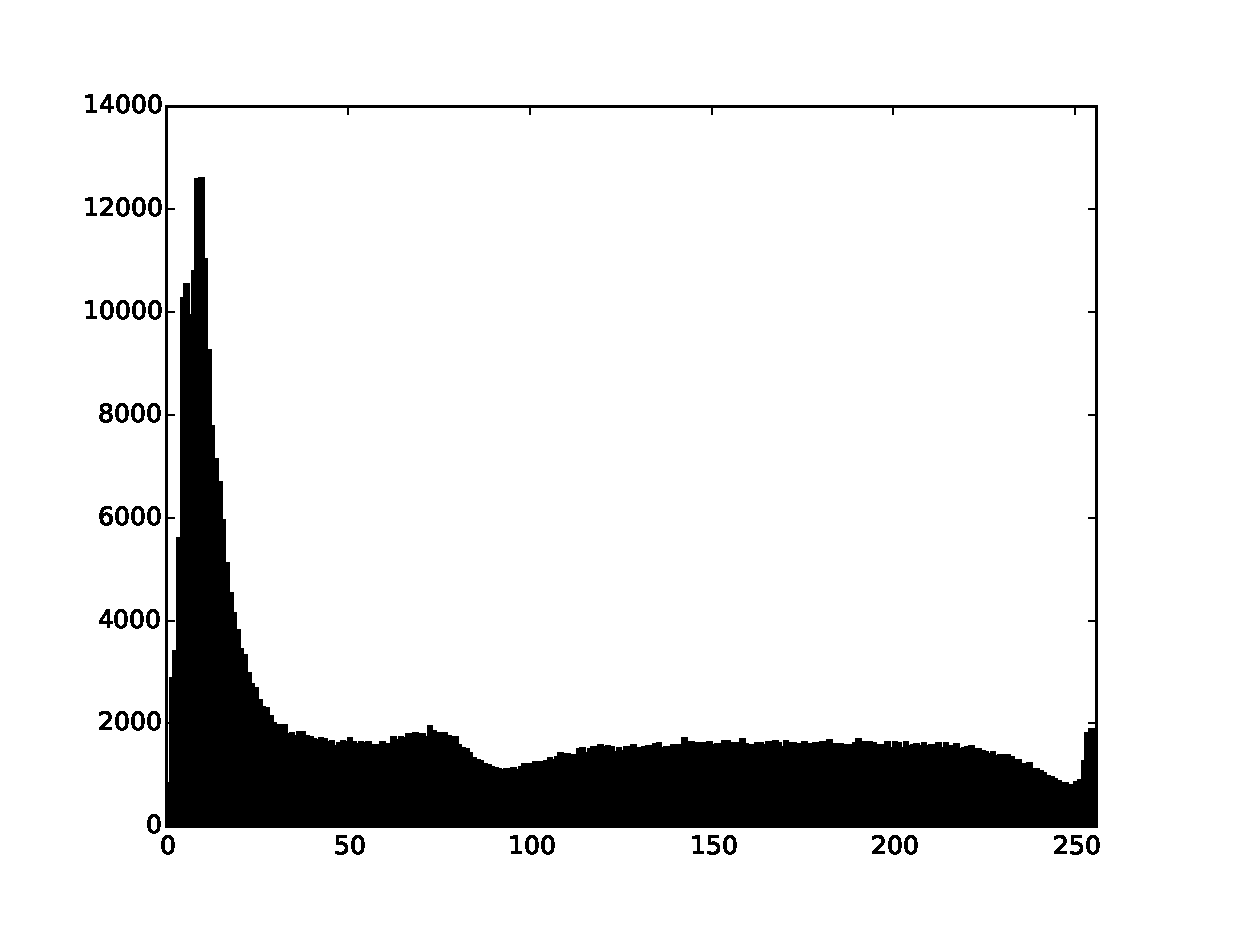
\includegraphics[width=0.520\linewidth]{bilder/moon_hist.eps}}
\end{figure}
\end{frame}

\begin{frame}{\insertsubsection}
\begin{figure}[T]
  \centering
  
\includegraphics[width=0.470\textwidth]{bilder/uniformnoise.png}
  \hfill
  \only<2>{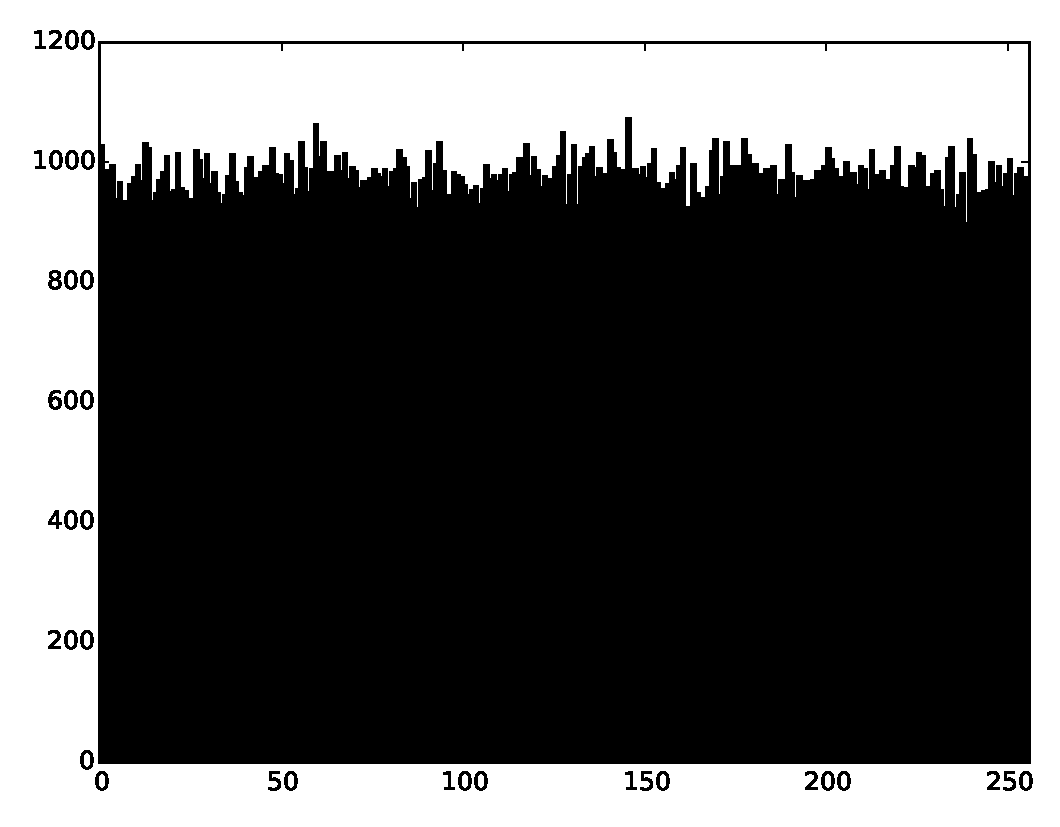
\includegraphics[width=0.520\linewidth]{bilder/uniformnoise_hist.eps}}
\end{figure}
\end{frame}

\subsection{Audiokompression}
\begin{frame}[<+->]{\insertsection}
\begin{witemize}
\item test
\end{witemize}
\end{frame}

\end{document}

%%%%%%%%%%%%%%%%%%%%%%%%%%%%%%%%%%%%%%%%%%%%%%%%%%%%%%%%%%%%

\begin{frame}[label=finalSlide]
  \label{LastPage}
  \begin{center}
    \vfill
    {\Large
    \textcolor{i6blue}{Danke für die Aufmerksamkeit!}
    }
     \vfill
     \inserttitle
    \vfill
    {\Large \insertauthor}
    \vfill
    \email{}
  \end{center}
\end{frame}
